% Options for packages loaded elsewhere
\PassOptionsToPackage{unicode}{hyperref}
\PassOptionsToPackage{hyphens}{url}
%
\documentclass[
  12pt,
  a4paper,
  DIV=11,
  numbers=noendperiod]{scrreprt}

\usepackage{amsmath,amssymb}
\usepackage{setspace}
\usepackage{iftex}
\ifPDFTeX
  \usepackage[T1]{fontenc}
  \usepackage[utf8]{inputenc}
  \usepackage{textcomp} % provide euro and other symbols
\else % if luatex or xetex
  \usepackage{unicode-math}
  \defaultfontfeatures{Scale=MatchLowercase}
  \defaultfontfeatures[\rmfamily]{Ligatures=TeX,Scale=1}
\fi
\usepackage{lmodern}
\ifPDFTeX\else  
    % xetex/luatex font selection
\fi
% Use upquote if available, for straight quotes in verbatim environments
\IfFileExists{upquote.sty}{\usepackage{upquote}}{}
\IfFileExists{microtype.sty}{% use microtype if available
  \usepackage[]{microtype}
  \UseMicrotypeSet[protrusion]{basicmath} % disable protrusion for tt fonts
}{}
\usepackage{xcolor}
\usepackage{svg}
\setlength{\emergencystretch}{3em} % prevent overfull lines
\setcounter{secnumdepth}{5}
% Make \paragraph and \subparagraph free-standing
\ifx\paragraph\undefined\else
  \let\oldparagraph\paragraph
  \renewcommand{\paragraph}[1]{\oldparagraph{#1}\mbox{}}
\fi
\ifx\subparagraph\undefined\else
  \let\oldsubparagraph\subparagraph
  \renewcommand{\subparagraph}[1]{\oldsubparagraph{#1}\mbox{}}
\fi

\usepackage{color}
\usepackage{fancyvrb}
\newcommand{\VerbBar}{|}
\newcommand{\VERB}{\Verb[commandchars=\\\{\}]}
\DefineVerbatimEnvironment{Highlighting}{Verbatim}{commandchars=\\\{\}}
% Add ',fontsize=\small' for more characters per line
\usepackage{framed}
\definecolor{shadecolor}{RGB}{241,243,245}
\newenvironment{Shaded}{\begin{snugshade}}{\end{snugshade}}
\newcommand{\AlertTok}[1]{\textcolor[rgb]{0.68,0.00,0.00}{#1}}
\newcommand{\AnnotationTok}[1]{\textcolor[rgb]{0.37,0.37,0.37}{#1}}
\newcommand{\AttributeTok}[1]{\textcolor[rgb]{0.40,0.45,0.13}{#1}}
\newcommand{\BaseNTok}[1]{\textcolor[rgb]{0.68,0.00,0.00}{#1}}
\newcommand{\BuiltInTok}[1]{\textcolor[rgb]{0.00,0.23,0.31}{#1}}
\newcommand{\CharTok}[1]{\textcolor[rgb]{0.13,0.47,0.30}{#1}}
\newcommand{\CommentTok}[1]{\textcolor[rgb]{0.37,0.37,0.37}{#1}}
\newcommand{\CommentVarTok}[1]{\textcolor[rgb]{0.37,0.37,0.37}{\textit{#1}}}
\newcommand{\ConstantTok}[1]{\textcolor[rgb]{0.56,0.35,0.01}{#1}}
\newcommand{\ControlFlowTok}[1]{\textcolor[rgb]{0.00,0.23,0.31}{#1}}
\newcommand{\DataTypeTok}[1]{\textcolor[rgb]{0.68,0.00,0.00}{#1}}
\newcommand{\DecValTok}[1]{\textcolor[rgb]{0.68,0.00,0.00}{#1}}
\newcommand{\DocumentationTok}[1]{\textcolor[rgb]{0.37,0.37,0.37}{\textit{#1}}}
\newcommand{\ErrorTok}[1]{\textcolor[rgb]{0.68,0.00,0.00}{#1}}
\newcommand{\ExtensionTok}[1]{\textcolor[rgb]{0.00,0.23,0.31}{#1}}
\newcommand{\FloatTok}[1]{\textcolor[rgb]{0.68,0.00,0.00}{#1}}
\newcommand{\FunctionTok}[1]{\textcolor[rgb]{0.28,0.35,0.67}{#1}}
\newcommand{\ImportTok}[1]{\textcolor[rgb]{0.00,0.46,0.62}{#1}}
\newcommand{\InformationTok}[1]{\textcolor[rgb]{0.37,0.37,0.37}{#1}}
\newcommand{\KeywordTok}[1]{\textcolor[rgb]{0.00,0.23,0.31}{#1}}
\newcommand{\NormalTok}[1]{\textcolor[rgb]{0.00,0.23,0.31}{#1}}
\newcommand{\OperatorTok}[1]{\textcolor[rgb]{0.37,0.37,0.37}{#1}}
\newcommand{\OtherTok}[1]{\textcolor[rgb]{0.00,0.23,0.31}{#1}}
\newcommand{\PreprocessorTok}[1]{\textcolor[rgb]{0.68,0.00,0.00}{#1}}
\newcommand{\RegionMarkerTok}[1]{\textcolor[rgb]{0.00,0.23,0.31}{#1}}
\newcommand{\SpecialCharTok}[1]{\textcolor[rgb]{0.37,0.37,0.37}{#1}}
\newcommand{\SpecialStringTok}[1]{\textcolor[rgb]{0.13,0.47,0.30}{#1}}
\newcommand{\StringTok}[1]{\textcolor[rgb]{0.13,0.47,0.30}{#1}}
\newcommand{\VariableTok}[1]{\textcolor[rgb]{0.07,0.07,0.07}{#1}}
\newcommand{\VerbatimStringTok}[1]{\textcolor[rgb]{0.13,0.47,0.30}{#1}}
\newcommand{\WarningTok}[1]{\textcolor[rgb]{0.37,0.37,0.37}{\textit{#1}}}

\providecommand{\tightlist}{%
  \setlength{\itemsep}{0pt}\setlength{\parskip}{0pt}}\usepackage{longtable,booktabs,array}
\usepackage{calc} % for calculating minipage widths
% Correct order of tables after \paragraph or \subparagraph
\usepackage{etoolbox}
\makeatletter
\patchcmd\longtable{\par}{\if@noskipsec\mbox{}\fi\par}{}{}
\makeatother
% Allow footnotes in longtable head/foot
\IfFileExists{footnotehyper.sty}{\usepackage{footnotehyper}}{\usepackage{footnote}}
\makesavenoteenv{longtable}
\usepackage{graphicx}
\makeatletter
\def\maxwidth{\ifdim\Gin@nat@width>\linewidth\linewidth\else\Gin@nat@width\fi}
\def\maxheight{\ifdim\Gin@nat@height>\textheight\textheight\else\Gin@nat@height\fi}
\makeatother
% Scale images if necessary, so that they will not overflow the page
% margins by default, and it is still possible to overwrite the defaults
% using explicit options in \includegraphics[width, height, ...]{}
\setkeys{Gin}{width=\maxwidth,height=\maxheight,keepaspectratio}
% Set default figure placement to htbp
\makeatletter
\def\fps@figure{htbp}
\makeatother

\usepackage{indentfirst}
\usepackage{float}
\floatplacement{figure}{H}
\IfFileExists{plex-otf.sty}{
  %% Full TeXlive
  \usepackage[
    % math,
    RM={Scale=0.94},SS={Scale=0.94},SScon={Scale=0.94},TT={Scale=MatchLowercase,FakeStretch=0.9},
    DefaultFeatures={Ligatures=Common}
  ]{plex-otf}
  % \usepackage[Scale=MatchUppercase]{juliamono}
}{
  %% TinyTeX
  \usepackage{libertine}
}
\KOMAoption{captions}{tableheading}
\makeatletter
\@ifpackageloaded{caption}{}{\usepackage{caption}}
\AtBeginDocument{%
\ifdefined\contentsname
  \renewcommand*\contentsname{Содержание}
\else
  \newcommand\contentsname{Содержание}
\fi
\ifdefined\listfigurename
  \renewcommand*\listfigurename{Список иллюстраций}
\else
  \newcommand\listfigurename{Список иллюстраций}
\fi
\ifdefined\listtablename
  \renewcommand*\listtablename{Список таблиц}
\else
  \newcommand\listtablename{Список таблиц}
\fi
\ifdefined\figurename
  \renewcommand*\figurename{Рисунок}
\else
  \newcommand\figurename{Рисунок}
\fi
\ifdefined\tablename
  \renewcommand*\tablename{Таблица}
\else
  \newcommand\tablename{Таблица}
\fi
}
\@ifpackageloaded{float}{}{\usepackage{float}}
\floatstyle{ruled}
\@ifundefined{c@chapter}{\newfloat{codelisting}{h}{lop}}{\newfloat{codelisting}{h}{lop}[chapter]}
\floatname{codelisting}{Список}
\newcommand*\listoflistings{\listof{codelisting}{Листинги}}
\makeatother
\makeatletter
\makeatother
\makeatletter
\@ifpackageloaded{caption}{}{\usepackage{caption}}
\@ifpackageloaded{subcaption}{}{\usepackage{subcaption}}
\makeatother
\ifLuaTeX
\usepackage[bidi=basic]{babel}
\else
\usepackage[bidi=default]{babel}
\fi
\babelprovide[main,import]{russian}
\babelprovide[import]{english}
% get rid of language-specific shorthands (see #6817):
\let\LanguageShortHands\languageshorthands
\def\languageshorthands#1{}
\ifLuaTeX
  \usepackage{selnolig}  % disable illegal ligatures
\fi
\usepackage[style=gost-numeric,backend=biber,langhook=extras,autolang=other*]{biblatex}
\addbibresource{bib/cite.bib}
\usepackage{csquotes}
\usepackage{bookmark}

\IfFileExists{xurl.sty}{\usepackage{xurl}}{} % add URL line breaks if available
\urlstyle{same} % disable monospaced font for URLs
\hypersetup{
  pdftitle={Отчёта по лабораторной работе 5},
  pdfauthor={Нджову Нелиа},
  pdflang={ru-RU},
  hidelinks,
  pdfcreator={LaTeX via pandoc}}

\title{Отчёта по лабораторной работе 5}
\usepackage{etoolbox}
\makeatletter
\providecommand{\subtitle}[1]{% add subtitle to \maketitle
  \apptocmd{\@title}{\par {\large #1 \par}}{}{}
}
\makeatother
\subtitle{Иммитационное моделирование}
\author{Нджову Нелиа}
\date{}

\begin{document}
\maketitle

\renewcommand*\contentsname{Содержание}
{
\setcounter{tocdepth}{1}
\tableofcontents
}
\listoffigures
\listoftables
\setstretch{1.5}
\chapter{Цель
работы}\label{ux446ux435ux43bux44c-ux440ux430ux431ux43eux442ux44b}

Цель этой лабораторной работы - моделирования Аппарат сетей петри.

\chapter{Задание}\label{ux437ux430ux434ux430ux43dux438ux435}

\begin{enumerate}
\def\labelenumi{\arabic{enumi}.}
\item
  Код модели
\item
  Базовые эксперименты
\item
  Анимация процесса
\item
  Итоговый отчёт
\end{enumerate}

\chapter{Теоретическое
введение}\label{ux442ux435ux43eux440ux435ux442ux438ux447ux435ux441ux43aux43eux435-ux432ux432ux435ux434ux435ux43dux438ux435}

\section{Сети
Петри}\label{ux441ux435ux442ux438-ux43fux435ux442ux440ux438}

Сеть Петри есть математический аппарат для моделирования дискретных
систем. в которых процессы происходят параллельно и асинхронно. Она
позволяет выявлять такие проблемы, как взаимная блокировка (deadlock).
Графически она представляется как двудольный ориентированный граф двух
типов вершин:

\begin{itemize}
\item
  Позиции (Places) суть пассивные элементы, описывающие состояние
  системы. Внутри позиции могут находиться фишки (tokens,
  неотрицательное целое число, указывающее на количество ресурсов)
\item
  Переходы (Transitions) суть активные элементы, описывающие события или
  действия системы. Они могут срабатывать, изменяя состояние модели.
\item
  Дуги соединяют позиции с переходами и показывают, какие ресурсы нужны
  для события и какие появляются после него.
\end{itemize}

\textbf{Правило срабатывания перехода:} Переход может сработать, если
каждая его входная позиция содержит хотя бы одну фишку. При срабатывании
из входных позиций фишки удаляются, а в выходные добавляются. Этот
процесс меняет маркировку сети, то есть её текущее состояние.

Сети Петри бывают детерминированными (описываются дифференциальными
уравнениями) и стохастическими (используют алгоритм Гиллеспи, где время
и выбор перехода определяются случайным образом).

\section{Задача «Обедающие
философы»}\label{ux437ux430ux434ux430ux447ux430-ux43eux431ux435ux434ux430ux44eux449ux438ux435-ux444ux438ux43bux43eux441ux43eux444ux44b}

Это классическая задача, иллюстрирующая проблему синхронизации в
параллельных системах.

\textbf{Постановка задачи:} За круглым столом сидят N философов (обычно
5). Перед каждым тарелка с едой. Между каждыми двумя соседними
философами лежит одна вилка. Всего вилок столько же, сколько философов.

\textbf{Правила:} Чтобы поесть, философу нужны две вилки --- левая и
правая. Если вилок нет, философ ждёт. Поев, философ кладёт вилки обратно
и возвращается к размышлениям.

\textbf{Проблема взаимной блокировки (deadlock):} Если все философы
одновременно возьмут левую вилку, то каждый будет держать одну вилку и
ждать правую, которая занята соседом. В результате никто не может есть
--- система замирает. Это и есть deadlock.

\textbf{Решение (арбитр):} Чтобы предотвратить deadlock, вводится арбитр
(официант), который разрешает есть не более чем N‑1 философам
одновременно. Это гарантирует, что хотя бы один философ всегда сможет
взять обе вилки, и система не блокируется.

\chapter{Выполнение лабораторной
работы}\label{ux432ux44bux43fux43eux43bux43dux435ux43dux438ux435-ux43bux430ux431ux43eux440ux430ux442ux43eux440ux43dux43eux439-ux440ux430ux431ux43eux442ux44b}

\section{1. Код
модели}\label{ux43aux43eux434-ux43cux43eux434ux435ux43bux438}

Я сначала создала файл src/DiningPhilosophers.jl.Потом скопировала
заданный скрипт в него. Скрипт содержить основные функции модели. Я
запускала и все работала хорошо(рис.1)

\begin{figure}

\centering{


\includegraphics[width=0.7\textwidth,height=\textheight]{image/pic1.png}

}

\caption{\label{fig-001}Код модели}

\end{figure}%

\section{2. Базовые
эксперименты}\label{ux431ux430ux437ux43eux432ux44bux435-ux44dux43aux441ux43fux435ux440ux438ux43cux435ux43dux442ux44b}

Я создала файл scripts/dining\_philosophers.jl.Потом скопировала
заданный скрипт в него. Скрипт выполняет основное моделирование и
сравнение двух вариантов сети Петри: классическая модель (без арбитра),
в которой возможна взаимная блокировка (deadlock). И модифицированная
модель с арбитром, которая должна предотвращать deadlock. Я
преобразавала код в литературный стиль и запускала.(рис.2)

\begin{figure}

\centering{


\includegraphics[width=0.7\textwidth,height=\textheight]{image/pic2.png}

}

\caption{\label{fig-002}Код базовых экспериментов}

\end{figure}%

После запуск, я получила две графики classic\_simulation.png и
arbiter\_simulation.png. Мы увидим четыре панели (Think, Hungry, Eat,
Fork) с динамикой для каждого философа.В классическом симуляторе
произошла взаимоблокировка, но в режиме арбитра этого не произошло(рис 3
и 4)

\begin{figure}

\centering{

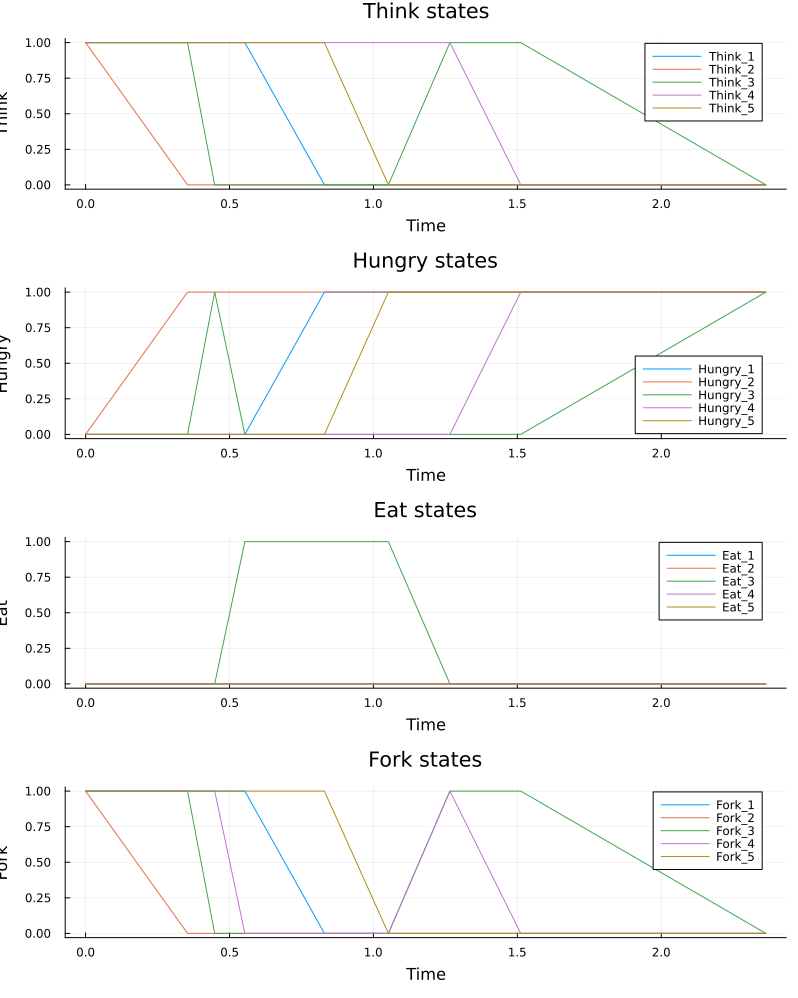
\includegraphics[width=0.7\textwidth,height=\textheight]{image/classic_simulation.png}

}

\caption{\label{fig-003}classic\_simulation.png}

\end{figure}%

\begin{figure}

\centering{

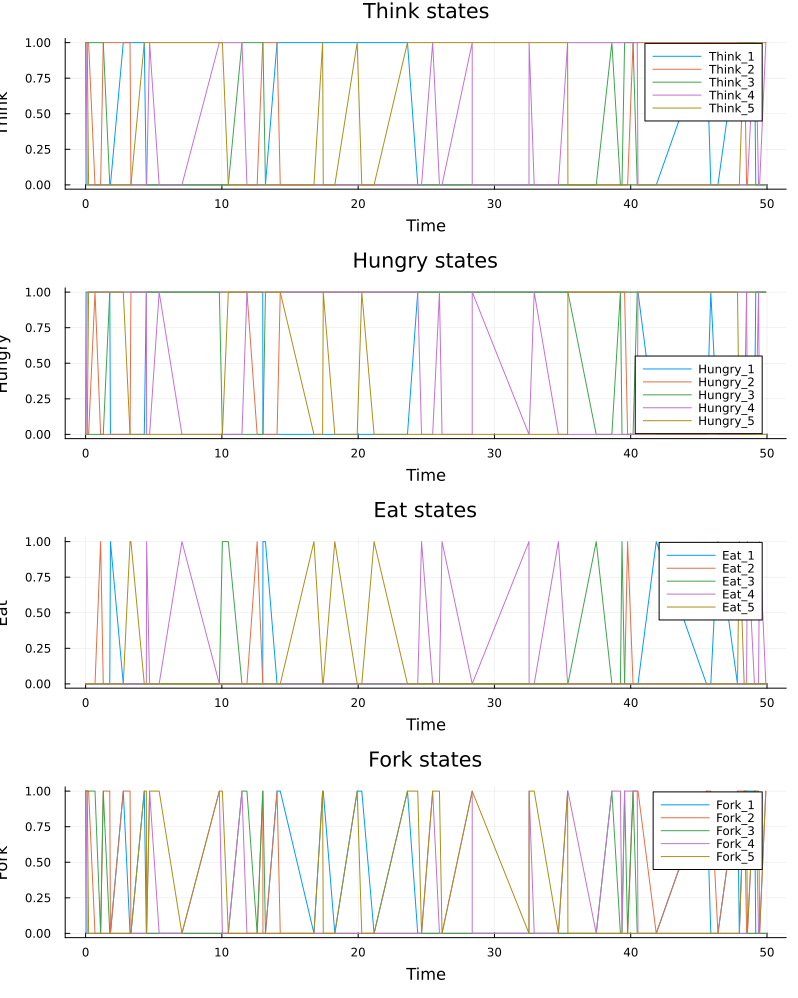
\includegraphics[width=0.7\textwidth,height=\textheight]{image/arbiter_simulation.png}

}

\caption{\label{fig-004}arbiter\_simulation.png}

\end{figure}%

Я генерировала файл jupyter, запускала все ячейки и всё работал
хорошо.(рис.5)

\begin{figure}

\centering{


\includegraphics[width=0.7\textwidth,height=\textheight]{image/pic6.png}

}

\caption{\label{fig-005}файл jupyter}

\end{figure}%

\textbf{\emph{Ниже приведен код, результаты расчетов и графики для кода
в файле scripts/dining\_philosophers.qmd}}

\section{Базовые
эксперименты}\label{ux431ux430ux437ux43eux432ux44bux435-ux44dux43aux441ux43fux435ux440ux438ux43cux435ux43dux442ux44b-1}

\textbf{Зачем нужен} Скрипт выполняет основное моделирование и сравнение
двух вариантов сети Петри: классическая модель (без арбитра), в которой
возможна взаимная блокировка (deadlock) и модифицированная модель с
арбитром, которая должна предотвращать deadlock.

\begin{Shaded}
\begin{Highlighting}[]
\ImportTok{using} \BuiltInTok{DrWatson}
\PreprocessorTok{@quickactivate} \StringTok{"project"}
\FunctionTok{include}\NormalTok{(}\FunctionTok{srcdir}\NormalTok{(}\StringTok{"DiningPhilosophers.jl"}\NormalTok{))}
\ImportTok{using} \BuiltInTok{.DiningPhilosophers}
\ImportTok{using} \BuiltInTok{DataFrames}\NormalTok{, }\BuiltInTok{CSV}\NormalTok{, }\BuiltInTok{Plots}
\end{Highlighting}
\end{Shaded}

\begin{verbatim}
┌ Warning: DrWatson could not find find a project file by recursively checking given `dir` and its parents. Returning `nothing` instead.
│ (given dir: /home/nelianjovu)
└ @ DrWatson ~/.julia/packages/DrWatson/2QF5p/src/project_setup.jl:84
WARNING: replacing module DiningPhilosophers.
WARNING: using DiningPhilosophers.build_classical_network in module Main conflicts with an existing identifier.
WARNING: using DiningPhilosophers.build_arbiter_network in module Main conflicts with an existing identifier.
WARNING: using DiningPhilosophers.simulate_stochastic in module Main conflicts with an existing identifier.
WARNING: using DiningPhilosophers.detect_deadlock in module Main conflicts with an existing identifier.
WARNING: using DiningPhilosophers.plot_marking_evolution in module Main conflicts with an existing identifier.
\end{verbatim}

Создаем классическую сеть Петри для N=5 философов с помощью
build\_classical\_network. Запускаем стохастическую симуляцию (алгоритм
Гиллеспи) на время tmax = 50.0.

\begin{Shaded}
\begin{Highlighting}[]
\NormalTok{N }\OperatorTok{=} \FloatTok{5}
\NormalTok{tmax }\OperatorTok{=} \FloatTok{50.0}

\FunctionTok{println}\NormalTok{(}\StringTok{"=== Классическая сеть (без арбитра) ==="}\NormalTok{)}
\NormalTok{net\_classic, u0\_classic, \_ }\OperatorTok{=} \FunctionTok{build\_classical\_network}\NormalTok{(N)}
\NormalTok{df\_classic }\OperatorTok{=} \FunctionTok{simulate\_stochastic}\NormalTok{(net\_classic, u0\_classic, tmax)}
\end{Highlighting}
\end{Shaded}

\begin{verbatim}
=== Классическая сеть (без арбитра) ===
\end{verbatim}

\begin{tabular}{r|cccccccccc}
    & time & Think\_1 & Think\_2 & Think\_3 & Think\_4 & Think\_5 & Hungry\_1 & Hungry\_2 & Hungry\_3 & \\
    \hline
    & Float64 & Float64 & Float64 & Float64 & Float64 & Float64 & Float64 & Float64 & Float64 & \\
    \hline
    1 & 0.0 & 1.0 & 1.0 & 1.0 & 1.0 & 1.0 & 0.0 & 0.0 & 0.0 & $\dots$ \\
    2 & 0.0875217 & 1.0 & 0.0 & 1.0 & 1.0 & 1.0 & 0.0 & 1.0 & 0.0 & $\dots$ \\
    3 & 0.324143 & 1.0 & 0.0 & 1.0 & 1.0 & 0.0 & 0.0 & 1.0 & 0.0 & $\dots$ \\
    4 & 0.535789 & 1.0 & 0.0 & 1.0 & 1.0 & 0.0 & 0.0 & 0.0 & 0.0 & $\dots$ \\
    5 & 0.591992 & 1.0 & 0.0 & 1.0 & 1.0 & 0.0 & 0.0 & 0.0 & 0.0 & $\dots$ \\
    6 & 0.628374 & 1.0 & 0.0 & 1.0 & 1.0 & 1.0 & 0.0 & 0.0 & 0.0 & $\dots$ \\
    7 & 0.966648 & 1.0 & 0.0 & 1.0 & 0.0 & 1.0 & 0.0 & 0.0 & 0.0 & $\dots$ \\
    8 & 1.05722 & 1.0 & 0.0 & 1.0 & 0.0 & 1.0 & 0.0 & 0.0 & 0.0 & $\dots$ \\
    9 & 1.07017 & 0.0 & 0.0 & 1.0 & 0.0 & 1.0 & 1.0 & 0.0 & 0.0 & $\dots$ \\
    10 & 1.11142 & 0.0 & 1.0 & 1.0 & 0.0 & 1.0 & 1.0 & 0.0 & 0.0 & $\dots$ \\
    11 & 2.1125 & 0.0 & 1.0 & 1.0 & 1.0 & 1.0 & 1.0 & 0.0 & 0.0 & $\dots$ \\
    12 & 2.69011 & 0.0 & 1.0 & 1.0 & 1.0 & 0.0 & 1.0 & 0.0 & 0.0 & $\dots$ \\
    13 & 2.82141 & 0.0 & 1.0 & 0.0 & 1.0 & 0.0 & 1.0 & 0.0 & 1.0 & $\dots$ \\
    14 & 3.25714 & 0.0 & 0.0 & 0.0 & 1.0 & 0.0 & 1.0 & 1.0 & 1.0 & $\dots$ \\
    15 & 3.46006 & 0.0 & 0.0 & 0.0 & 1.0 & 0.0 & 1.0 & 1.0 & 0.0 & $\dots$ \\
    16 & 4.26298 & 0.0 & 0.0 & 1.0 & 1.0 & 0.0 & 1.0 & 1.0 & 0.0 & $\dots$ \\
    17 & 4.3116 & 0.0 & 0.0 & 1.0 & 1.0 & 0.0 & 1.0 & 0.0 & 0.0 & $\dots$ \\
    18 & 4.69192 & 0.0 & 0.0 & 1.0 & 0.0 & 0.0 & 1.0 & 0.0 & 0.0 & $\dots$ \\
    19 & 6.80485 & 0.0 & 1.0 & 1.0 & 0.0 & 0.0 & 1.0 & 0.0 & 0.0 & $\dots$ \\
    20 & 7.07096 & 0.0 & 1.0 & 0.0 & 0.0 & 0.0 & 1.0 & 0.0 & 1.0 & $\dots$ \\
    21 & 8.65562 & 0.0 & 0.0 & 0.0 & 0.0 & 0.0 & 1.0 & 1.0 & 1.0 & $\dots$ \\
\end{tabular}

Сохраняем полную историю маркировок в CSV-файл (dining\_classic.csv).

\begin{Shaded}
\begin{Highlighting}[]
\NormalTok{CSV.}\FunctionTok{write}\NormalTok{(}\FunctionTok{datadir}\NormalTok{(}\StringTok{"dining\_classic.csv"}\NormalTok{), df\_classic)}
\end{Highlighting}
\end{Shaded}

\begin{verbatim}
"/home/nelianjovu/work/study/2026-1/2026-1==study--simulationmod/2026-1--study--simulationmod/labs/lab05/project/data/dining_classic.csv"
\end{verbatim}

Анализируем последнее состояние на предмет deadlock с помощью
detect\_deadlock и выводит результат в консоль.

\begin{Shaded}
\begin{Highlighting}[]
\NormalTok{dead }\OperatorTok{=} \FunctionTok{detect\_deadlock}\NormalTok{(df\_classic, net\_classic)}
\FunctionTok{println}\NormalTok{(}\StringTok{"Deadlock обнаружен: }\SpecialCharTok{$}\NormalTok{dead}\StringTok{"}\NormalTok{)}
\end{Highlighting}
\end{Shaded}

\begin{verbatim}
Deadlock обнаружен: true
\end{verbatim}

Строим графики эволюции маркировки по всем позициям (Think, Hungry, Eat,
Fork) и сохраняет их как classic\_simulation.png.

\begin{Shaded}
\begin{Highlighting}[]
\NormalTok{plot\_classic }\OperatorTok{=} \FunctionTok{plot\_marking\_evolution}\NormalTok{(df\_classic, N)}
\FunctionTok{savefig}\NormalTok{(}\FunctionTok{plotsdir}\NormalTok{(}\StringTok{"classic\_simulation.png"}\NormalTok{))}
\end{Highlighting}
\end{Shaded}

\begin{verbatim}
"/home/nelianjovu/work/study/2026-1/2026-1==study--simulationmod/2026-1--study--simulationmod/labs/lab05/project/plots/classic_simulation.png"
\end{verbatim}

Повторяем для сети с арбитром (build\_arbiter\_network), сохраняя
результаты в dining\_arbiter.csv и arbiter\_simulation.png.

\begin{Shaded}
\begin{Highlighting}[]
\FunctionTok{println}\NormalTok{(}\StringTok{"}\SpecialCharTok{\textbackslash{}n}\StringTok{=== Сеть с арбитром ==="}\NormalTok{)}
\NormalTok{net\_arb, u0\_arb, \_ }\OperatorTok{=} \FunctionTok{build\_arbiter\_network}\NormalTok{(N)}
\NormalTok{df\_arb }\OperatorTok{=} \FunctionTok{simulate\_stochastic}\NormalTok{(net\_arb, u0\_arb, tmax)}
\NormalTok{CSV.}\FunctionTok{write}\NormalTok{(}\FunctionTok{datadir}\NormalTok{(}\StringTok{"dining\_arbiter.csv"}\NormalTok{), df\_arb)}
\NormalTok{dead\_arb }\OperatorTok{=} \FunctionTok{detect\_deadlock}\NormalTok{(df\_arb, net\_arb)}
\FunctionTok{println}\NormalTok{(}\StringTok{"Deadlock обнаружен: }\SpecialCharTok{$}\NormalTok{dead\_arb}\StringTok{"}\NormalTok{)}
\NormalTok{plot\_arb }\OperatorTok{=} \FunctionTok{plot\_marking\_evolution}\NormalTok{(df\_arb, N)}
\FunctionTok{savefig}\NormalTok{(}\FunctionTok{plotsdir}\NormalTok{(}\StringTok{"arbiter\_simulation.png"}\NormalTok{))}
\end{Highlighting}
\end{Shaded}

\begin{verbatim}

=== Сеть с арбитром ===
Deadlock обнаружен: false
\end{verbatim}

\begin{verbatim}
"/home/nelianjovu/work/study/2026-1/2026-1==study--simulationmod/2026-1--study--simulationmod/labs/lab05/project/plots/arbiter_simulation.png"
\end{verbatim}

Я изменила количество философов в эксперименте, я использовала N = 2 и N
= 10. И в обоих экспериментах тупик возник в классическом моделировании,
но не в произвольном моделировании(рис.6)

\begin{figure}

\centering{


\includegraphics[width=0.7\textwidth,height=\textheight]{image/pic12.png}

}

\caption{\label{fig-006}изменения количества философов}

\end{figure}%

Я генерировала файл jupyter, запускала все ячейки и всё работал
хорошо.(рис.7)

\begin{figure}

\centering{


\includegraphics[width=0.7\textwidth,height=\textheight]{image/pic14.png}

}

\caption{\label{fig-007}файл jupyter}

\end{figure}%

\textbf{\emph{Ниже приведен код, результаты расчетов и графики для кода
в файле scripts/dining\_philosophers\_params.qmd}}

\section{Базовые
эксперименты}\label{ux431ux430ux437ux43eux432ux44bux435-ux44dux43aux441ux43fux435ux440ux438ux43cux435ux43dux442ux44b-2}

\textbf{Зачем нужен} Скрипт выполняет основное моделирование и сравнение
двух вариантов сети Петри: классическая модель (без арбитра), в которой
возможна взаимная блокировка (deadlock) и модифицированная модель с
арбитром, которая должна предотвращать deadlock.

\begin{Shaded}
\begin{Highlighting}[]
\ImportTok{using} \BuiltInTok{DrWatson}
\PreprocessorTok{@quickactivate} \StringTok{"project"}
\FunctionTok{include}\NormalTok{(}\FunctionTok{srcdir}\NormalTok{(}\StringTok{"DiningPhilosophers.jl"}\NormalTok{))}
\ImportTok{using} \BuiltInTok{.DiningPhilosophers}
\ImportTok{using} \BuiltInTok{DataFrames}\NormalTok{, }\BuiltInTok{CSV}\NormalTok{, }\BuiltInTok{Plots}
\end{Highlighting}
\end{Shaded}

\begin{verbatim}
┌ Warning: DrWatson could not find find a project file by recursively checking given `dir` and its parents. Returning `nothing` instead.
│ (given dir: /home/nelianjovu)
└ @ DrWatson ~/.julia/packages/DrWatson/2QF5p/src/project_setup.jl:84
WARNING: replacing module DiningPhilosophers.
WARNING: using DiningPhilosophers.build_classical_network in module Main conflicts with an existing identifier.
WARNING: using DiningPhilosophers.build_arbiter_network in module Main conflicts with an existing identifier.
WARNING: using DiningPhilosophers.simulate_stochastic in module Main conflicts with an existing identifier.
WARNING: using DiningPhilosophers.detect_deadlock in module Main conflicts with an existing identifier.
WARNING: using DiningPhilosophers.plot_marking_evolution in module Main conflicts with an existing identifier.
\end{verbatim}

Создаем классическую сеть Петри для N=2 и N1=10 философов с помощью
build\_classical\_network. Запускаем стохастическую симуляцию (алгоритм
Гиллеспи) на время tmax = 50.0.

\begin{Shaded}
\begin{Highlighting}[]
\NormalTok{N }\OperatorTok{=} \FloatTok{2}
\NormalTok{N1 }\OperatorTok{=} \FloatTok{10}
\NormalTok{tmax }\OperatorTok{=} \FloatTok{50.0}

\FunctionTok{println}\NormalTok{(}\StringTok{"=== Классическая сеть (без арбитра) ==="}\NormalTok{)}
\NormalTok{net\_classic, u0\_classic, \_ }\OperatorTok{=} \FunctionTok{build\_classical\_network}\NormalTok{(N)}
\NormalTok{net\_classic1, u0\_classic1, \_ }\OperatorTok{=} \FunctionTok{build\_classical\_network}\NormalTok{(N1)}
\NormalTok{df\_classic }\OperatorTok{=} \FunctionTok{simulate\_stochastic}\NormalTok{(net\_classic, u0\_classic, tmax)}
\NormalTok{df\_classic1 }\OperatorTok{=} \FunctionTok{simulate\_stochastic}\NormalTok{(net\_classic1, u0\_classic1, tmax)}
\end{Highlighting}
\end{Shaded}

\begin{verbatim}
=== Классическая сеть (без арбитра) ===
\end{verbatim}

\begin{tabular}{r|cccccccccc}
    & time & Think\_1 & Think\_2 & Think\_3 & Think\_4 & Think\_5 & Think\_6 & Think\_7 & Think\_8 & \\
    \hline
    & Float64 & Float64 & Float64 & Float64 & Float64 & Float64 & Float64 & Float64 & Float64 & \\
    \hline
    1 & 0.0 & 1.0 & 1.0 & 1.0 & 1.0 & 1.0 & 1.0 & 1.0 & 1.0 & $\dots$ \\
    2 & 0.0427495 & 1.0 & 1.0 & 1.0 & 1.0 & 1.0 & 1.0 & 1.0 & 0.0 & $\dots$ \\
    3 & 0.0723963 & 1.0 & 1.0 & 1.0 & 1.0 & 0.0 & 1.0 & 1.0 & 0.0 & $\dots$ \\
    4 & 0.111753 & 1.0 & 1.0 & 1.0 & 1.0 & 0.0 & 1.0 & 1.0 & 0.0 & $\dots$ \\
    5 & 0.206046 & 1.0 & 1.0 & 0.0 & 1.0 & 0.0 & 1.0 & 1.0 & 0.0 & $\dots$ \\
    6 & 0.23235 & 1.0 & 1.0 & 0.0 & 1.0 & 0.0 & 0.0 & 1.0 & 0.0 & $\dots$ \\
    7 & 0.63024 & 1.0 & 1.0 & 0.0 & 1.0 & 0.0 & 0.0 & 1.0 & 0.0 & $\dots$ \\
    8 & 0.689216 & 1.0 & 1.0 & 0.0 & 0.0 & 0.0 & 0.0 & 1.0 & 0.0 & $\dots$ \\
    9 & 0.782221 & 1.0 & 1.0 & 0.0 & 0.0 & 0.0 & 0.0 & 0.0 & 0.0 & $\dots$ \\
    10 & 0.894808 & 1.0 & 0.0 & 0.0 & 0.0 & 0.0 & 0.0 & 0.0 & 0.0 & $\dots$ \\
    11 & 1.52887 & 1.0 & 0.0 & 0.0 & 0.0 & 0.0 & 0.0 & 0.0 & 0.0 & $\dots$ \\
    12 & 3.19943 & 1.0 & 0.0 & 0.0 & 0.0 & 0.0 & 0.0 & 0.0 & 0.0 & $\dots$ \\
    13 & 3.237 & 0.0 & 0.0 & 0.0 & 0.0 & 0.0 & 0.0 & 0.0 & 0.0 & $\dots$ \\
    14 & 3.92789 & 0.0 & 0.0 & 0.0 & 0.0 & 0.0 & 0.0 & 0.0 & 0.0 & $\dots$ \\
\end{tabular}

Сохраняем полную историю маркировок в CSV-файл (dining\_classic.csv).

\begin{Shaded}
\begin{Highlighting}[]
\NormalTok{CSV.}\FunctionTok{write}\NormalTok{(}\FunctionTok{datadir}\NormalTok{(}\StringTok{"dining\_classic(N=2).csv"}\NormalTok{), df\_classic)}
\NormalTok{CSV.}\FunctionTok{write}\NormalTok{(}\FunctionTok{datadir}\NormalTok{(}\StringTok{"dining\_classic(N=10).csv"}\NormalTok{), df\_classic1)}
\end{Highlighting}
\end{Shaded}

\begin{verbatim}
"/home/nelianjovu/work/study/2026-1/2026-1==study--simulationmod/2026-1--study--simulationmod/labs/lab05/project/data/dining_classic(N=10).csv"
\end{verbatim}

Анализируем последнее состояние на предмет deadlock с помощью
detect\_deadlock и выводит результат в консоль.

\begin{Shaded}
\begin{Highlighting}[]
\NormalTok{dead }\OperatorTok{=} \FunctionTok{detect\_deadlock}\NormalTok{(df\_classic, net\_classic)}
\NormalTok{dead1 }\OperatorTok{=} \FunctionTok{detect\_deadlock}\NormalTok{(df\_classic1, net\_classic1)}
\FunctionTok{println}\NormalTok{(}\StringTok{"Deadlock обнаружен(N=2): }\SpecialCharTok{$}\NormalTok{dead}\StringTok{"}\NormalTok{)}
\FunctionTok{println}\NormalTok{(}\StringTok{"Deadlock обнаружен(N=10): }\SpecialCharTok{$}\NormalTok{dead1}\StringTok{"}\NormalTok{)}
\end{Highlighting}
\end{Shaded}

\begin{verbatim}
Deadlock обнаружен(N=2): true
Deadlock обнаружен(N=10): true
\end{verbatim}

Строим графики эволюции маркировки по всем позициям (Think, Hungry, Eat,
Fork) и сохраняет их как classic\_simulation.png.

\begin{Shaded}
\begin{Highlighting}[]
\NormalTok{plot\_classic }\OperatorTok{=} \FunctionTok{plot\_marking\_evolution}\NormalTok{(df\_classic, N)}
\NormalTok{plot\_classic1 }\OperatorTok{=} \FunctionTok{plot\_marking\_evolution}\NormalTok{(df\_classic1, N1)}
\FunctionTok{savefig}\NormalTok{(}\FunctionTok{plotsdir}\NormalTok{(}\StringTok{"classic\_simulation(N=2).png"}\NormalTok{))}
\FunctionTok{savefig}\NormalTok{(}\FunctionTok{plotsdir}\NormalTok{(}\StringTok{"classic\_simulation(N=10).png"}\NormalTok{))}
\end{Highlighting}
\end{Shaded}

\begin{verbatim}
"/home/nelianjovu/work/study/2026-1/2026-1==study--simulationmod/2026-1--study--simulationmod/labs/lab05/project/plots/classic_simulation(N=10).png"
\end{verbatim}

Повторяем для сети с арбитром (build\_arbiter\_network), сохраняя
результаты в dining\_arbiter.csv и arbiter\_simulation.png.

\begin{Shaded}
\begin{Highlighting}[]
\FunctionTok{println}\NormalTok{(}\StringTok{"}\SpecialCharTok{\textbackslash{}n}\StringTok{=== Сеть с арбитром ==="}\NormalTok{)}
\NormalTok{net\_arb, u0\_arb, \_ }\OperatorTok{=} \FunctionTok{build\_arbiter\_network}\NormalTok{(N)}
\NormalTok{df\_arb }\OperatorTok{=} \FunctionTok{simulate\_stochastic}\NormalTok{(net\_arb, u0\_arb, tmax)}
\NormalTok{CSV.}\FunctionTok{write}\NormalTok{(}\FunctionTok{datadir}\NormalTok{(}\StringTok{"dining\_arbiter(N=2).csv"}\NormalTok{), df\_arb)}
\NormalTok{dead\_arb }\OperatorTok{=} \FunctionTok{detect\_deadlock}\NormalTok{(df\_arb, net\_arb)}
\FunctionTok{println}\NormalTok{(}\StringTok{"Deadlock обнаружен(N=2): }\SpecialCharTok{$}\NormalTok{dead\_arb}\StringTok{"}\NormalTok{)}
\NormalTok{plot\_arb }\OperatorTok{=} \FunctionTok{plot\_marking\_evolution}\NormalTok{(df\_arb, N)}
\FunctionTok{savefig}\NormalTok{(}\FunctionTok{plotsdir}\NormalTok{(}\StringTok{"arbiter\_simulation(N=2).png"}\NormalTok{))}

\NormalTok{net\_arb1, u0\_arb1, \_ }\OperatorTok{=} \FunctionTok{build\_arbiter\_network}\NormalTok{(N1)}
\NormalTok{df\_arb1 }\OperatorTok{=} \FunctionTok{simulate\_stochastic}\NormalTok{(net\_arb1, u0\_arb1, tmax)}
\NormalTok{CSV.}\FunctionTok{write}\NormalTok{(}\FunctionTok{datadir}\NormalTok{(}\StringTok{"dining\_arbiter(N=10).csv"}\NormalTok{), df\_arb1)}
\NormalTok{dead\_arb1 }\OperatorTok{=} \FunctionTok{detect\_deadlock}\NormalTok{(df\_arb1, net\_arb1)}
\FunctionTok{println}\NormalTok{(}\StringTok{"Deadlock обнаружен(N=10): }\SpecialCharTok{$}\NormalTok{dead\_arb1}\StringTok{"}\NormalTok{)}
\NormalTok{plot\_arb1 }\OperatorTok{=} \FunctionTok{plot\_marking\_evolution}\NormalTok{(df\_arb1, N1)}
\FunctionTok{savefig}\NormalTok{(}\FunctionTok{plotsdir}\NormalTok{(}\StringTok{"arbiter\_simulation(N=10).png"}\NormalTok{))}
\end{Highlighting}
\end{Shaded}

\begin{verbatim}

=== Сеть с арбитром ===
Deadlock обнаружен(N=2): false
Deadlock обнаружен(N=10): false
\end{verbatim}

\begin{verbatim}
"/home/nelianjovu/work/study/2026-1/2026-1==study--simulationmod/2026-1--study--simulationmod/labs/lab05/project/plots/arbiter_simulation(N=10).png"
\end{verbatim}

\section{3. Анимация
процесса}\label{ux430ux43dux438ux43cux430ux446ux438ux44f-ux43fux440ux43eux446ux435ux441ux441ux430}

Я создала файл scripts/dining\_philosophers\_animation.jl.Потом
скопировала заданный скрипт в него. Скрипт используется для наглядной
демонстрации динамики работы сети Петри во времени. Анимация позволяет
увидеть, как меняется маркировка (фишки) в каждой позиции, и особенно
наглядно показывает возникновение deadlock в классической модели(рис.8)

\begin{figure}

\centering{


\includegraphics[width=0.7\textwidth,height=\textheight]{image/pic15.png}

}

\caption{\label{fig-008}Код Анимации процесса}

\end{figure}%

\section{4. Итоговый
отчёт}\label{ux438ux442ux43eux433ux43eux432ux44bux439-ux43eux442ux447ux451ux442}

Я создала файл scripts/dining\_philosophers\_report.jl.Потом скопировала
заданный скрипт в него. Скрипт используется для сравнительного анализа
двух моделей (с арбитром и без) по одному ключевому показателю --- числу
философов, находящихся в состоянии «Ест» (Eat\_i). Скрипт генерирует
сводный график.(рис.9)

\begin{figure}

\centering{

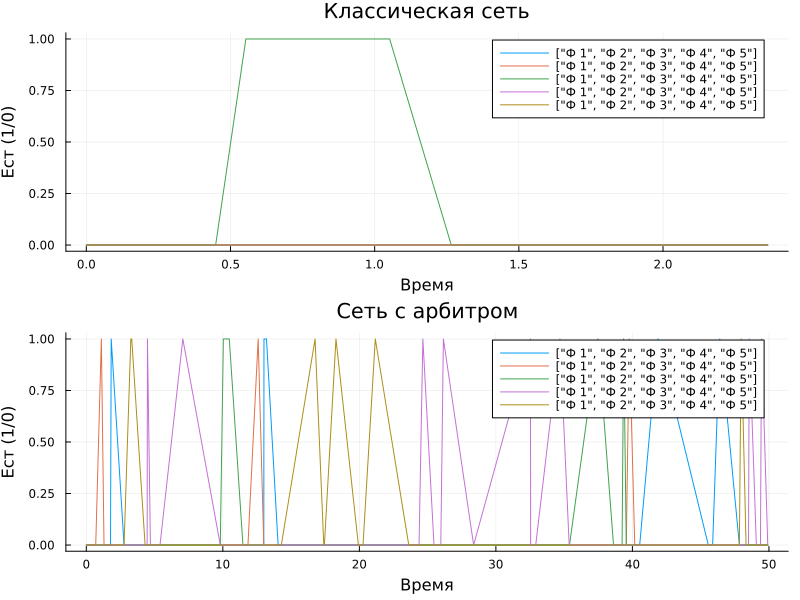
\includegraphics[width=0.7\textwidth,height=\textheight]{image/final_report.png}

}

\caption{\label{fig-009}Код Итогового отчёта}

\end{figure}%

Я преобразовала код в литературный стиль, генерировала файл jupyter и
выполнила все ячейки(рис.10)

\begin{figure}

\centering{


\includegraphics[width=0.7\textwidth,height=\textheight]{image/pic19.png}

}

\caption{\label{fig-010}файл jupyter}

\end{figure}%

\textbf{\emph{Ниже приведен код, результаты расчетов и графики для кода
в файле scripts/scripts/dining\_philosophers\_report.qmd}}

\section{Итоговый
отчёт}\label{ux438ux442ux43eux433ux43eux432ux44bux439-ux43eux442ux447ux451ux442-1}

\textbf{Зачем нужен:} Для сравнительного анализа двух моделей (с
арбитром и без) по одному ключевому показателю --- числу философов,
находящихся в состоянии «Ест» (Eat\_i). Скрипт генерирует сводный
график.

\begin{Shaded}
\begin{Highlighting}[]
\ImportTok{using} \BuiltInTok{DrWatson}
\PreprocessorTok{@quickactivate} \StringTok{"project"}
\ImportTok{using} \BuiltInTok{DataFrames}\NormalTok{, }\BuiltInTok{CSV}\NormalTok{, }\BuiltInTok{Plots}
\FunctionTok{gr}\NormalTok{(fmt}\OperatorTok{=:}\NormalTok{png)}
\end{Highlighting}
\end{Shaded}

\begin{verbatim}
┌ Warning: DrWatson could not find find a project file by recursively checking given `dir` and its parents. Returning `nothing` instead.
│ (given dir: /home/nelianjovu)
└ @ DrWatson ~/.julia/packages/DrWatson/2QF5p/src/project_setup.jl:84
\end{verbatim}

\begin{verbatim}
Plots.GRBackend()
\end{verbatim}

Загружает ранее сохранённые CSV-файлы (dining\_classic.csv и
dining\_arbiter.csv) из папки data/.

\begin{Shaded}
\begin{Highlighting}[]
\NormalTok{df\_classic }\OperatorTok{=}\NormalTok{ CSV.}\FunctionTok{read}\NormalTok{(}\FunctionTok{datadir}\NormalTok{(}\StringTok{"dining\_classic.csv"}\NormalTok{), DataFrame)}
\NormalTok{df\_arbiter }\OperatorTok{=}\NormalTok{ CSV.}\FunctionTok{read}\NormalTok{(}\FunctionTok{datadir}\NormalTok{(}\StringTok{"dining\_arbiter.csv"}\NormalTok{), DataFrame)}
\NormalTok{N }\OperatorTok{=} \FloatTok{5}
\end{Highlighting}
\end{Shaded}

\begin{verbatim}
5
\end{verbatim}

Столбцы для состояния \enquote{Ест}

\begin{Shaded}
\begin{Highlighting}[]
\NormalTok{eat\_cols }\OperatorTok{=}\NormalTok{ [}\FunctionTok{Symbol}\NormalTok{(}\StringTok{"Eat\_}\SpecialCharTok{$}\NormalTok{i}\StringTok{"}\NormalTok{) for i }\OperatorTok{=} \FloatTok{1}\OperatorTok{:}\NormalTok{N]}
\end{Highlighting}
\end{Shaded}

\begin{verbatim}
5-element Vector{Symbol}:
 :Eat_1
 :Eat_2
 :Eat_3
 :Eat_4
 :Eat_5
\end{verbatim}

Строит два временных графика (один под другим): динамику «едящих»
философов для классической сети и для сети с арбитром.

\begin{Shaded}
\begin{Highlighting}[]
\NormalTok{p1 }\OperatorTok{=} \FunctionTok{plot}\NormalTok{(}
\NormalTok{    df\_classic.time,}
    \FunctionTok{Matrix}\NormalTok{(df\_classic[}\OperatorTok{:}\NormalTok{, eat\_cols]),}
\NormalTok{    label }\OperatorTok{=}\NormalTok{ [}\StringTok{"Ф }\SpecialCharTok{$}\NormalTok{i}\StringTok{"}\NormalTok{ for i }\OperatorTok{=} \FloatTok{1}\OperatorTok{:}\NormalTok{N],}
\NormalTok{    xlabel }\OperatorTok{=} \StringTok{"Время"}\NormalTok{,}
\NormalTok{    ylabel }\OperatorTok{=} \StringTok{"Ест (1/0)"}\NormalTok{,}
\NormalTok{    title }\OperatorTok{=} \StringTok{"Классическая сеть"}\NormalTok{,}
\NormalTok{    )}

\NormalTok{p2 }\OperatorTok{=} \FunctionTok{plot}\NormalTok{(}
\NormalTok{    df\_arbiter.time,}
    \FunctionTok{Matrix}\NormalTok{(df\_arbiter[}\OperatorTok{:}\NormalTok{, eat\_cols]),}
\NormalTok{    label }\OperatorTok{=}\NormalTok{ [}\StringTok{"Ф }\SpecialCharTok{$}\NormalTok{i}\StringTok{"}\NormalTok{ for i }\OperatorTok{=} \FloatTok{1}\OperatorTok{:}\NormalTok{N],}
\NormalTok{    xlabel }\OperatorTok{=} \StringTok{"Время"}\NormalTok{,}
\NormalTok{    ylabel }\OperatorTok{=} \StringTok{"Ест (1/0)"}\NormalTok{,}
\NormalTok{    title }\OperatorTok{=} \StringTok{"Сеть с арбитром"}\NormalTok{,}
\NormalTok{    )}
\end{Highlighting}
\end{Shaded}

\includesvg{simmod-lab05-report (Нджову Нелиа)_files/figure-pdf/cell-18-output-1.svg}

Сохраняет объединённый график как final\_report.png в папку plots/.

\begin{Shaded}
\begin{Highlighting}[]
\NormalTok{p\_final }\OperatorTok{=} \FunctionTok{plot}\NormalTok{(p1, p2, layout }\OperatorTok{=}\NormalTok{ (}\FloatTok{2}\NormalTok{, }\FloatTok{1}\NormalTok{), size }\OperatorTok{=}\NormalTok{ (}\FloatTok{800}\NormalTok{, }\FloatTok{600}\NormalTok{))}
\FunctionTok{savefig}\NormalTok{(}\FunctionTok{plotsdir}\NormalTok{(}\StringTok{"final\_report.png"}\NormalTok{))}
\FunctionTok{println}\NormalTok{(}\StringTok{"Отчёт сохранён в plots/final\_report.png"}\NormalTok{)}
\end{Highlighting}
\end{Shaded}

\begin{verbatim}
Отчёт сохранён в plots/final_report.png
\end{verbatim}

Я изменила скрипт, чтобы он работал при N = 2 и N = 10(рис. 11 и 12)

\begin{figure}

\centering{

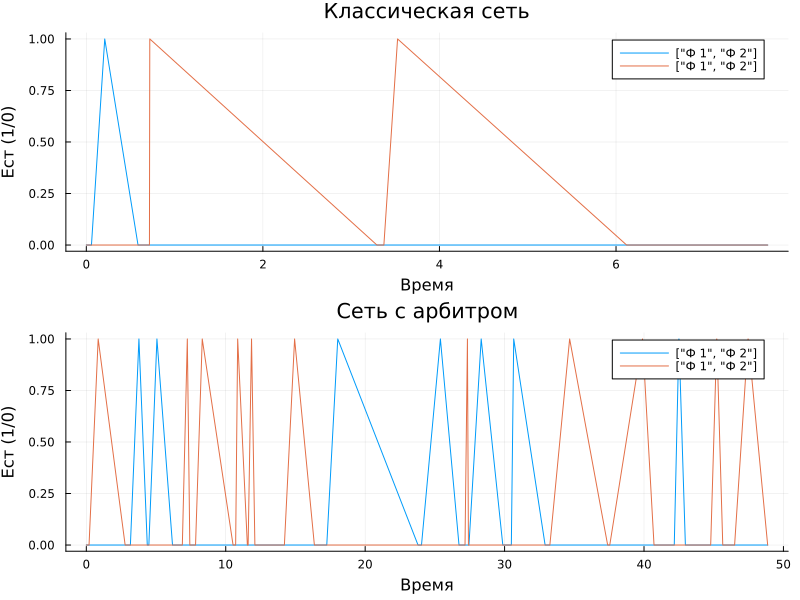
\includegraphics[width=0.7\textwidth,height=\textheight]{image/final_report(N=2).png}

}

\caption{\label{fig-011}Код Итогового отчёта(N=2)}

\end{figure}%

\begin{figure}

\centering{

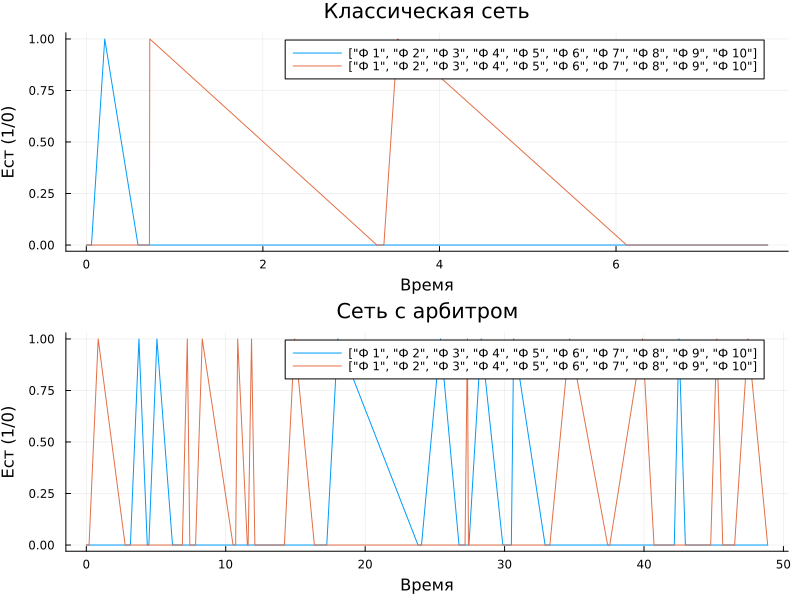
\includegraphics[width=0.7\textwidth,height=\textheight]{image/final_report(N=10).png}

}

\caption{\label{fig-012}Код Итогового отчёта(N=10)}

\end{figure}%

Я преобразовала код в литературный стиль, генерировала файл jupyter и
выполнила все ячейки(рис.13)

\begin{figure}

\centering{


\includegraphics[width=0.7\textwidth,height=\textheight]{image/pic22.png}

}

\caption{\label{fig-013}файл jupyter}

\end{figure}%

\textbf{\emph{Ниже приведен код, результаты расчетов и графики для кода
в файле scripts/scripts/dining\_philosophers\_report\_param.qmd}}

\section{Итоговый
отчёт}\label{ux438ux442ux43eux433ux43eux432ux44bux439-ux43eux442ux447ux451ux442-2}

\textbf{Зачем нужен:} Для сравнительного анализа двух моделей (с
арбитром и без) по одному ключевому показателю --- числу философов,
находящихся в состоянии «Ест» (Eat\_i). Скрипт генерирует сводный
график.

\begin{Shaded}
\begin{Highlighting}[]
\ImportTok{using} \BuiltInTok{DrWatson}
\PreprocessorTok{@quickactivate} \StringTok{"project"}
\ImportTok{using} \BuiltInTok{DataFrames}\NormalTok{, }\BuiltInTok{CSV}\NormalTok{, }\BuiltInTok{Plots}
\FunctionTok{gr}\NormalTok{(fmt}\OperatorTok{=:}\NormalTok{png)}
\end{Highlighting}
\end{Shaded}

\begin{verbatim}
┌ Warning: DrWatson could not find find a project file by recursively checking given `dir` and its parents. Returning `nothing` instead.
│ (given dir: /home/nelianjovu)
└ @ DrWatson ~/.julia/packages/DrWatson/2QF5p/src/project_setup.jl:84
\end{verbatim}

\begin{verbatim}
Plots.GRBackend()
\end{verbatim}

Загружает ранее сохранённые CSV-файлы (dining\_classic.csv и
dining\_arbiter.csv) из папки data/.

\begin{Shaded}
\begin{Highlighting}[]
\NormalTok{df\_classic }\OperatorTok{=}\NormalTok{ CSV.}\FunctionTok{read}\NormalTok{(}\FunctionTok{datadir}\NormalTok{(}\StringTok{"dining\_classic(N=2).csv"}\NormalTok{), DataFrame)}
\NormalTok{df\_arbiter }\OperatorTok{=}\NormalTok{ CSV.}\FunctionTok{read}\NormalTok{(}\FunctionTok{datadir}\NormalTok{(}\StringTok{"dining\_arbiter(N=2).csv"}\NormalTok{), DataFrame)}
\NormalTok{N }\OperatorTok{=} \FloatTok{2}

\NormalTok{df\_classic1 }\OperatorTok{=}\NormalTok{ CSV.}\FunctionTok{read}\NormalTok{(}\FunctionTok{datadir}\NormalTok{(}\StringTok{"dining\_classic(N=10).csv"}\NormalTok{), DataFrame)}
\NormalTok{df\_arbiter1 }\OperatorTok{=}\NormalTok{ CSV.}\FunctionTok{read}\NormalTok{(}\FunctionTok{datadir}\NormalTok{(}\StringTok{"dining\_arbiter(N=10).csv"}\NormalTok{), DataFrame)}
\NormalTok{N1 }\OperatorTok{=} \FloatTok{10}
\end{Highlighting}
\end{Shaded}

\begin{verbatim}
10
\end{verbatim}

Столбцы для состояния \enquote{Ест}

\begin{Shaded}
\begin{Highlighting}[]
\NormalTok{eat\_cols }\OperatorTok{=}\NormalTok{ [}\FunctionTok{Symbol}\NormalTok{(}\StringTok{"Eat\_}\SpecialCharTok{$}\NormalTok{i}\StringTok{"}\NormalTok{) for i }\OperatorTok{=} \FloatTok{1}\OperatorTok{:}\NormalTok{N]}
\NormalTok{eat\_cols1 }\OperatorTok{=}\NormalTok{ [}\FunctionTok{Symbol}\NormalTok{(}\StringTok{"Eat\_}\SpecialCharTok{$}\NormalTok{i}\StringTok{"}\NormalTok{) for i }\OperatorTok{=} \FloatTok{1}\OperatorTok{:}\NormalTok{N1]}
\end{Highlighting}
\end{Shaded}

\begin{verbatim}
10-element Vector{Symbol}:
 :Eat_1
 :Eat_2
 :Eat_3
 :Eat_4
 :Eat_5
 :Eat_6
 :Eat_7
 :Eat_8
 :Eat_9
 :Eat_10
\end{verbatim}

Строит два временных графика (один под другим): динамику «едящих»
философов для классической сети и для сети с арбитром. N = 2

\begin{Shaded}
\begin{Highlighting}[]
\NormalTok{p1 }\OperatorTok{=} \FunctionTok{plot}\NormalTok{(}
\NormalTok{    df\_classic.time,}
    \FunctionTok{Matrix}\NormalTok{(df\_classic[}\OperatorTok{:}\NormalTok{, eat\_cols]),}
\NormalTok{    label }\OperatorTok{=}\NormalTok{ [}\StringTok{"Ф }\SpecialCharTok{$}\NormalTok{i}\StringTok{"}\NormalTok{ for i }\OperatorTok{=} \FloatTok{1}\OperatorTok{:}\NormalTok{N],}
\NormalTok{    xlabel }\OperatorTok{=} \StringTok{"Время"}\NormalTok{,}
\NormalTok{    ylabel }\OperatorTok{=} \StringTok{"Ест (1/0)"}\NormalTok{,}
\NormalTok{    title }\OperatorTok{=} \StringTok{"Классическая сеть"}\NormalTok{,}
\NormalTok{    )}

\NormalTok{p2 }\OperatorTok{=} \FunctionTok{plot}\NormalTok{(}
\NormalTok{    df\_arbiter.time,}
    \FunctionTok{Matrix}\NormalTok{(df\_arbiter[}\OperatorTok{:}\NormalTok{, eat\_cols]),}
\NormalTok{    label }\OperatorTok{=}\NormalTok{ [}\StringTok{"Ф }\SpecialCharTok{$}\NormalTok{i}\StringTok{"}\NormalTok{ for i }\OperatorTok{=} \FloatTok{1}\OperatorTok{:}\NormalTok{N],}
\NormalTok{    xlabel }\OperatorTok{=} \StringTok{"Время"}\NormalTok{,}
\NormalTok{    ylabel }\OperatorTok{=} \StringTok{"Ест (1/0)"}\NormalTok{,}
\NormalTok{    title }\OperatorTok{=} \StringTok{"Сеть с арбитром"}\NormalTok{,}
\NormalTok{    )}
\end{Highlighting}
\end{Shaded}

\includesvg{simmod-lab05-report (Нджову Нелиа)_files/figure-pdf/cell-23-output-1.svg}

N = 10

\begin{Shaded}
\begin{Highlighting}[]
\NormalTok{p3 }\OperatorTok{=} \FunctionTok{plot}\NormalTok{(}
\NormalTok{    df\_classic.time,}
    \FunctionTok{Matrix}\NormalTok{(df\_classic[}\OperatorTok{:}\NormalTok{, eat\_cols]),}
\NormalTok{    label }\OperatorTok{=}\NormalTok{ [}\StringTok{"Ф }\SpecialCharTok{$}\NormalTok{i}\StringTok{"}\NormalTok{ for i }\OperatorTok{=} \FloatTok{1}\OperatorTok{:}\NormalTok{N1],}
\NormalTok{    xlabel }\OperatorTok{=} \StringTok{"Время"}\NormalTok{,}
\NormalTok{    ylabel }\OperatorTok{=} \StringTok{"Ест (1/0)"}\NormalTok{,}
\NormalTok{    title }\OperatorTok{=} \StringTok{"Классическая сеть"}\NormalTok{,}
\NormalTok{    )}

\NormalTok{p4 }\OperatorTok{=} \FunctionTok{plot}\NormalTok{(}
\NormalTok{    df\_arbiter.time,}
    \FunctionTok{Matrix}\NormalTok{(df\_arbiter[}\OperatorTok{:}\NormalTok{, eat\_cols]),}
\NormalTok{    label }\OperatorTok{=}\NormalTok{ [}\StringTok{"Ф }\SpecialCharTok{$}\NormalTok{i}\StringTok{"}\NormalTok{ for i }\OperatorTok{=} \FloatTok{1}\OperatorTok{:}\NormalTok{N1],}
\NormalTok{    xlabel }\OperatorTok{=} \StringTok{"Время"}\NormalTok{,}
\NormalTok{    ylabel }\OperatorTok{=} \StringTok{"Ест (1/0)"}\NormalTok{,}
\NormalTok{    title }\OperatorTok{=} \StringTok{"Сеть с арбитром"}\NormalTok{,}
\NormalTok{    )}
\end{Highlighting}
\end{Shaded}

\includesvg{simmod-lab05-report (Нджову Нелиа)_files/figure-pdf/cell-24-output-1.svg}

Сохраняет объединённый график как final\_report.png в папку plots/.

\begin{Shaded}
\begin{Highlighting}[]
\NormalTok{p\_final }\OperatorTok{=} \FunctionTok{plot}\NormalTok{(p1, p2, layout }\OperatorTok{=}\NormalTok{ (}\FloatTok{2}\NormalTok{, }\FloatTok{1}\NormalTok{), size }\OperatorTok{=}\NormalTok{ (}\FloatTok{800}\NormalTok{, }\FloatTok{600}\NormalTok{))}
\FunctionTok{savefig}\NormalTok{(}\FunctionTok{plotsdir}\NormalTok{(}\StringTok{"final\_report(N=2).png"}\NormalTok{))}

\NormalTok{p\_final1 }\OperatorTok{=} \FunctionTok{plot}\NormalTok{(p3, p4, layout }\OperatorTok{=}\NormalTok{ (}\FloatTok{2}\NormalTok{, }\FloatTok{1}\NormalTok{), size }\OperatorTok{=}\NormalTok{ (}\FloatTok{800}\NormalTok{, }\FloatTok{600}\NormalTok{))}
\FunctionTok{savefig}\NormalTok{(}\FunctionTok{plotsdir}\NormalTok{(}\StringTok{"final\_report(N=10).png"}\NormalTok{))}
\FunctionTok{println}\NormalTok{(}\StringTok{"Отчёт сохранён в plots/final\_report.png"}\NormalTok{)}
\end{Highlighting}
\end{Shaded}

\begin{verbatim}
Отчёт сохранён в plots/final_report.png
\end{verbatim}

\chapter{Выводы}\label{ux432ux44bux432ux43eux434ux44b}

Выполняя эту лабораторную работу, научилась моделировать аппарат сетей
Петри.


\printbibliography


\end{document}
